\documentclass[conference]{IEEEtran}
\IEEEoverridecommandlockouts
% The preceding line is only needed to identify funding in the first footnote. If that is unneeded, please comment it out.
\usepackage{cite}
\usepackage{amsmath,amssymb,amsfonts}
\usepackage{algorithmic}
\usepackage{graphicx}
\usepackage{textcomp}
\usepackage{xcolor}
\usepackage{multirow}
\newcommand{\quotes}[1]{``#1''}
\def\BibTeX{{\rm B\kern-.05em{\sc i\kern-.025em b}\kern-.08em
    T\kern-.1667em\lower.7ex\hbox{E}\kern-.125emX}}
\begin{document}

\title{A Review on Machine Learning Algorithms for Automatic Requirements Classification}

\author{\IEEEauthorblockN{J. Manuel Pérez-Verdejo}
\IEEEauthorblockA{\textit{School of Statistics and Informatics} \\
\textit{Universidad Veracruzana}\\
Xalapa, Veracruz, México \\
manuel.vrdjo@gmail.com}
\and
\IEEEauthorblockN{Ángel Juan Sánchez-García}
\IEEEauthorblockA{\textit{School of Statistics and Informatics} \\
\textit{Universidad Veracruzana}\\
Xalapa, Veracruz, México \\
angesanchez@uv.mx}
\and
\IEEEauthorblockN{Jorge Octavio Ocharán-Hernández}
\IEEEauthorblockA{\textit{School of Statistics and Informatics} \\
\textit{Universidad Veracruzana}\\
Xalapa, Veracruz, México \\
jocharan@uv.mx}
}

\maketitle

\begin{abstract}
The development of quality software begins with the correct identification of the system needs. These requirements represent the basis of the subsequent activities in the software life cycle. The correct identification of these requirements in their different categories impacts on the actions taken to meet them. However, this classification can be often time-consuming or error-prone when it comes to large-scale systems, so different proposals have been made to assist in this process automatically. This systematic literature review identifies those applications of Machine Learning techniques in the classification of software requirements. In this regard, 13 articles were identified, from which relevant information on the applied algorithms, their training process, and their evaluation metrics are analyzed. From the results obtained, it is identified that the most recurrent classification algorithms featured on the identified studies are Naïve Bayes, Decision Trees, and Natural Language Processing algorithms. The most frequent training datasets are academic databases and collected user reviews.
\end{abstract}

\begin{IEEEkeywords}
Requirements Engineering, Requirements Classification, Machine Learning, Classification, Systematic Literature Review
\end{IEEEkeywords}

\section{Introduction}
\label{introduction}

Requirements Engineering (RE), conceived as a sub-discipline dedicated to encompassing the capabilities and attributes that a system must fulfill \cite{Wiegers2013}, involves several of the most relevant activities within the software development process. Moreover, its elicitation, analysis, specification, and validation stages \cite{Kotonya:1998:REP:552009} represent a set of activities focused on understanding the customer's needs regarding the software to be developed.

In this regard, it is in the requirements analysis where the customer input results of the elicitation methods are refined into classified requirements for tracing. Thus, in this phase, the requirements analyst classifies the user statements into nine different categories of requirements \cite{Wiegers2013}: business requirements, external interface requirements, quality attributes, data requirements, functional requirements, solution ideas, business rules, user requirements, and constraints.

However, this activity including the elicitation process is usually time-consuming and error-prone \cite{METH20131695}, therefore the application of new techniques that assist in this type of task means a field of opportunity. Thus, the use of machine learning becomes a viable alternative, by dedicating its work to the construction of programs able to automatically improve with the experience \cite{Mitchell:1997:ML:541177}.

With the aim to provide initial insight into the application of machine learning strategies to automatically classify software requirements, the present study carries out a systematic literature review, to portrait the state of the art of this field.

This paper is organized as follows. Section \ref{method} describes the research method followed to conduct the review in machine learning algorithms for requirements classification. In Section \ref{conducting}, the conducting process of the systematic review is described, as well as the primary studies found. Section \ref{results} presents the results obtained from data extraction and synthesis performed in the review. In section \ref{discussion} the results found are discussed. Finally, the conclusions and the identified insights are summarized in section \ref{conclusions}.

\section{Research Method}
\label{method}

The research method followed to conduct the review was based on the guidelines described by Kitchenham and Charters \cite{Kitchenham2007}. Hence, the procedure was divided into three stages: (1) planning, (2) execution, and (3) reporting, which is shown in section \ref{results}.

\subsection{Planning}

In this stage, the following activities that guided the review are described: the establishment of the research questions, definition of the data sources and the search strategy, and the definition of the selection criteria. Those are further described in the following subsections.

\subsubsection{Research Questions}

The research questions elaborated to carry on the systematic review are:

\begin{itemize}
  \item \textit{RQ1: Which machine learning algorithms have been adopted to classify requirements?}
  \item \textit{RQ2: What metrics have been used to measure the performance of those algorithms?}
  \item \textit{RQ3: What kind of software projects have been used to train those algorithms?}
  \item \textit{RQ4: Which requirements categories are the most frequent to train those algorithms?}
\end{itemize}

The goal of RQ1 is to find evidence of the application of specific machine learning techniques in the RE, specifically in the classification of requirements. However, the classes to be identified are expected as belonging to one of the requirement categories identified by Wiegers and Beatty \cite{Wiegers2013}. Regarding RQ2, it establishes the goal of identifying how to evaluate the proposed models, for this way of comparing results between them.

The RQ3 is determined to understand the domain in which the model proposals are focused. Therefore, it is possible to know the necessary means to adopt general models to specific domains. On the other hand, RQ4 is focused to know the categories of requirements that have been considered for the application of those classifiers.

\subsubsection{Search Process}

The search for studies was carried out in four academic databases, access to which is provided by the National Consortium of Scientific and Technological Information Resources (abbreviated CONRICyt in Spanish). Table \ref{tab:selected-databases} shows their names and pages.

\begin{table}[!htbp]
% table caption is above the table
\caption{Selected Databases}
\label{tab:selected-databases}       % Give a unique label
% For LaTeX tables use
\begin{tabular}{p{4cm}p{4cm}}
\hline\noalign{\smallskip}
Database & URL  \\
\noalign{\smallskip}\hline\noalign{\smallskip}
IEEEXplore & https://ieeexplore.ieee.org \\
ACM Digital Library & https://dl.acm.org \\
Science Direct & https://www.sciencedirect.com \\
SpringerLink & https://link.springer.com \\
\noalign{\smallskip}\hline
\end{tabular}
\end{table}

Additionally, the search process was carried out guided by the three following search strings: 

\begin{itemize}
  \item\quotes{Requirements Engineering} AND \quotes{Machine Learning}
  \item\quotes{Software Requirements Elicitation} AND (\quotes{Machine Learning} OR \quotes{Machine Learning Model})
  \item(\quotes{Machine Learning} OR \quotes{Machine Learning Model}) AND \quotes{Software Requirements Classification}
\end{itemize}

The first is related to identifying applications belonging to the machine learning area in Requirements Engineering, this in order to find a more general approach for these implementations. The second search string is established as the analysis phase is considered to be the phase immediately following the elicitation \cite{Wiegers2013}. Finally, the third search string is meant to directly identify requirements classification papers.

\subsubsection{Study Selection}

The searches were performed by applying the first stage of inclusion and exclusion criteria directly to the search engines of the academic databases, in order to reduce results beyond the review scope. With this regard, publications that met the following requirements were collected:

\begin{itemize}
  \item{Published between 2010 and 2019}
  \item{Is either a journal or a conference paper}
  \item{Is accessible}
  \item{Features the search terms either in the title or the abstract}
\end{itemize}

\subsubsection{Primary Studies Selection}

On this matter, inclusion and exclusion criteria were established for the selection of primary studies. The process of applying these criteria was carried out in two stages. The criteria within the stages are described in Table \ref{tab:inclusion-exclusion-criteria}.

\begin{table}[!htbp]
\caption{Inclusion and Exclusion Criteria}
\begin{center}
\label{tab:inclusion-exclusion-criteria}       % Give a unique label
% For LaTeX tables use
\begin{tabular}{p{1.3cm}p{3cm}p{3cm}}
    \hline\noalign{\smallskip}
    Stage & Inclusion Criteria & Exclusion Criteria  \\
    \noalign{\smallskip}\hline\noalign{\smallskip}
    \multirow{2}{1.3cm}{Second Stage}& 1. The paper is published in English. & 1. The paper is duplicated. \\ & 2. Either the title or the abstract leads to answer at least one research question & 2. Neither the title nor the abstract features at least one of the search terms \\
    \hline\noalign{\smallskip}
    Third Stage & 1. The domain of the study is focused on the application of machine learning in Software Requirements Engineering. & 1. The domain of the study does not consist in the application of some technique of requirements classification in any of the categories defined in \cite{Wiegers2013}. \\
    \hline\noalign{\smallskip}
\end{tabular}
\end{center}
\end{table}

\subsubsection{Data Extraction}

From each identified article once all the criteria have been applied, the following information is collected: title, authors, publication year, source, type of publication, reference, keywords, abstract, and the answer to the research questions addressed.
Additionally, topic modeling analysis is performed to identify the most frequent terms and trends throughout the identified studies. For this procedure, the transcribed version of the articles featured on their web pages was required. If it wasn't available, the content was extracted directly from the file.

\section{Conducting}
\label{conducting}

Once the searches were made with the predefined criteria in the academic search engines, 325 articles were obtained. From these publications, a superficial review was made regarding the titles and abstracts, to identify potential answers to the research questions. As a result of this preliminary analysis, 55 papers were identified. Moreover, those documents that had already been identified, either in another database or with another search string were excluded, the last to avoid repeated articles. Finally, a detailed reading of the remaining 38 studies was made, until all those that met the criteria were identified, resulting in a total of 13 articles. Figure \ref{fig:rsl} describes this process and Table \ref{tab:studies} shows the studies included in the review, their publication year and source.

\begin{figure}[!htbp]
    \center{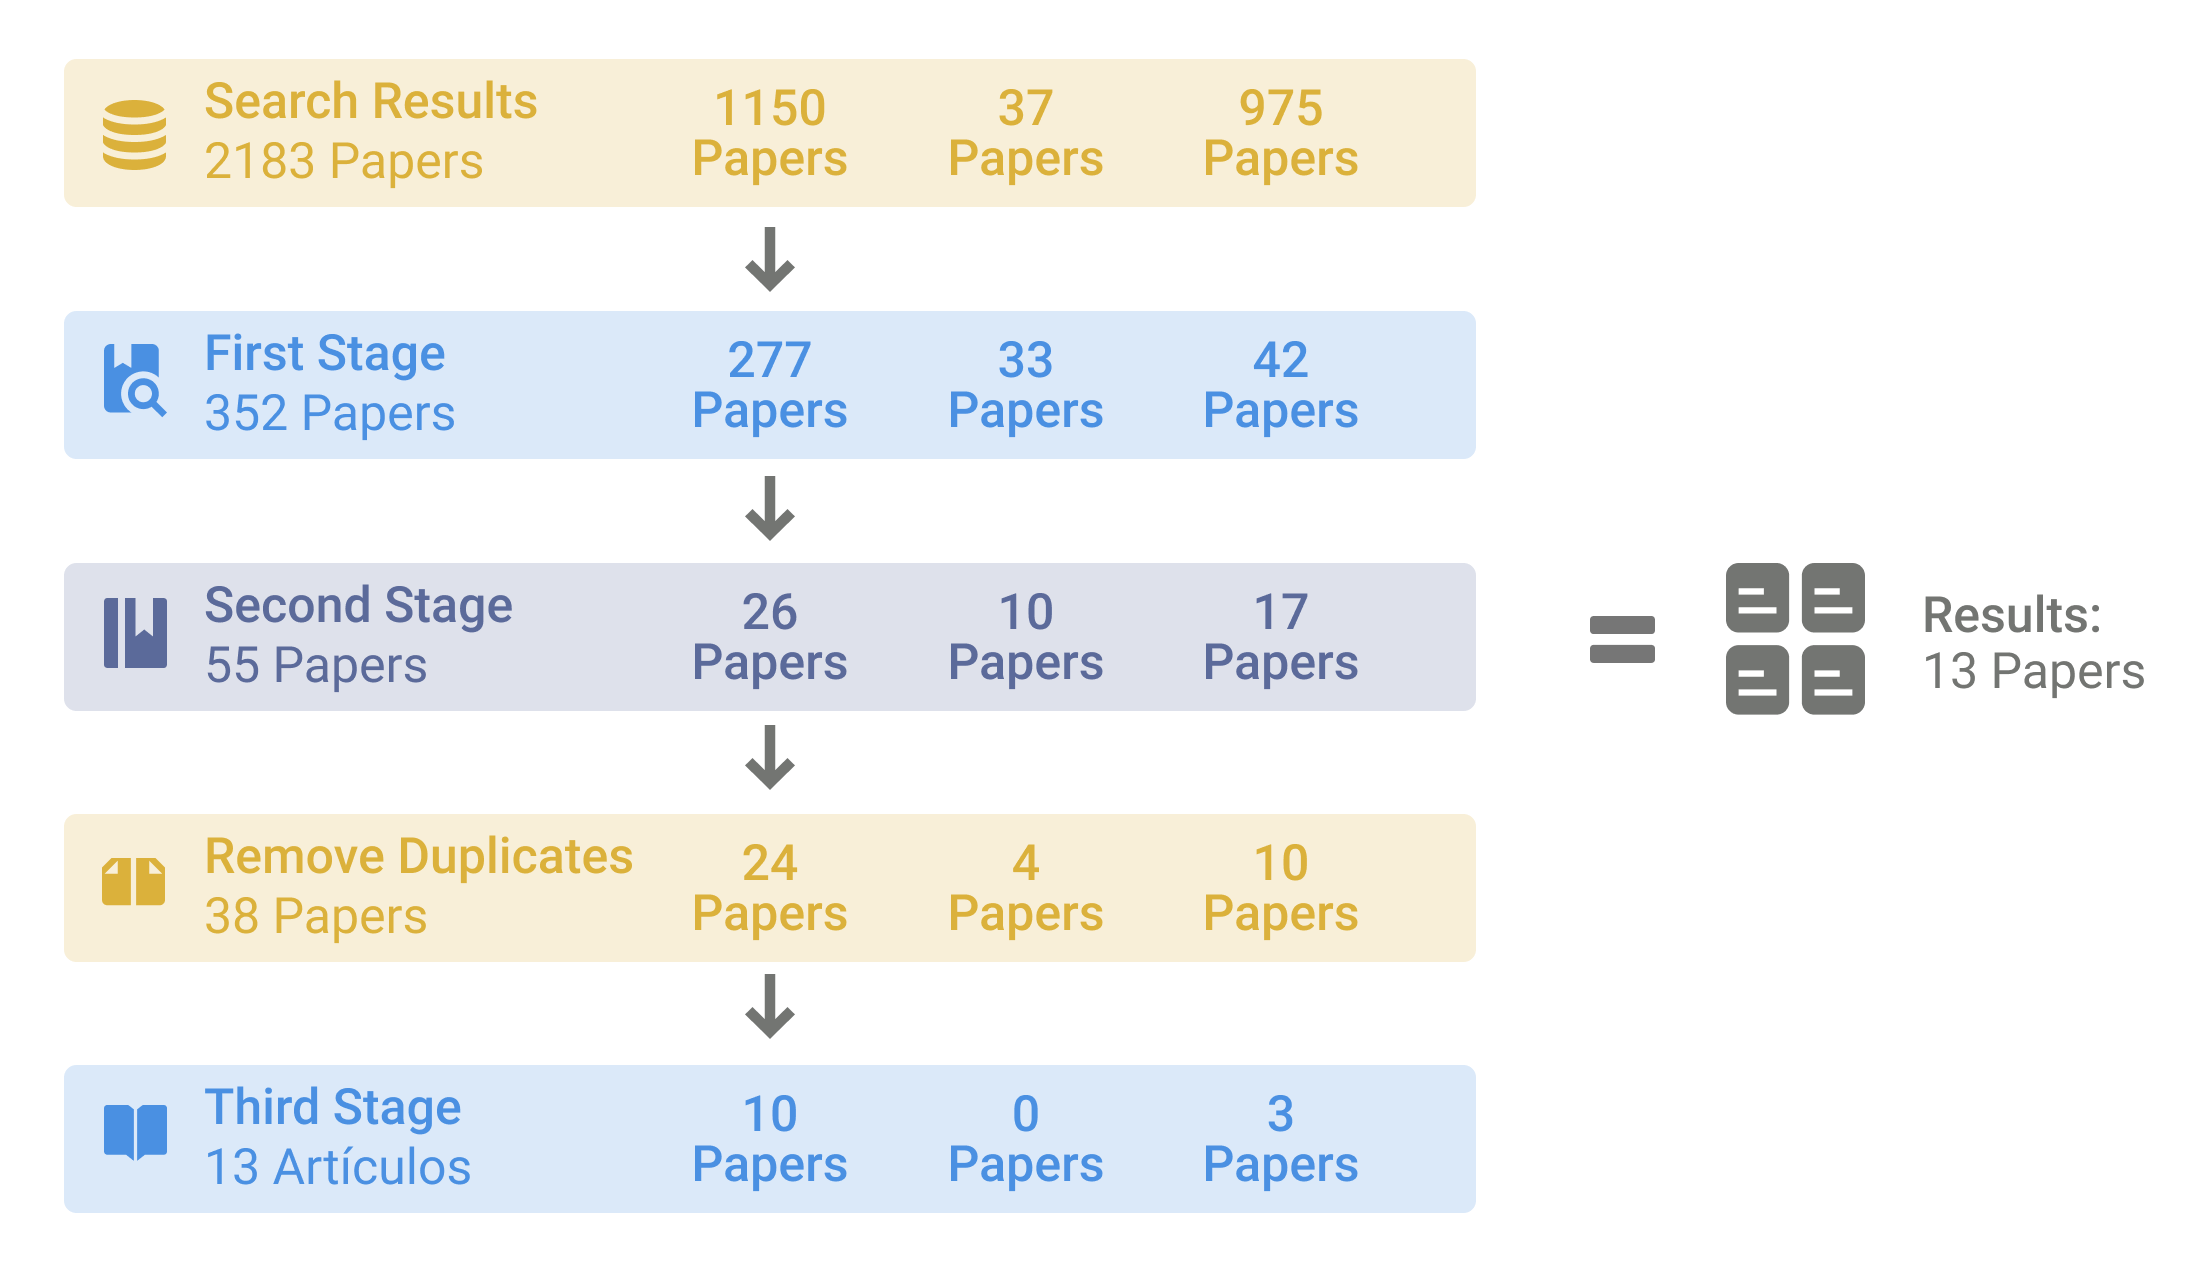
\includegraphics[scale=0.113]
        {Figures/rsl.png}}
    \caption{\label{fig:rsl}Number of papers included during the study selection process}
\end{figure}

\begin{table}[!htbp]
% table caption is above the table
\caption{Systematic review studies}
\label{tab:studies}       % Give a unique label
% For LaTeX tables use
\begin{tabular}{p{0.1cm}p{2cm}p{0.4cm}p{4.4cm}}
\hline\noalign{\smallskip}
ID & Author & Date & Source \\
\noalign{\smallskip}\hline\noalign{\smallskip}
S1 & Abad et al. \cite{8049172} & 2017 & International Requirements Engineering Conference \\
S2 & Baker et al. \cite{8754214} & 2019 & Computer Software and Applications Conference \\
S3 & Dekhtyar and Fong \cite{8049170} & 2017 & International Requirements Engineering Conference \\
S4 & Iqbal, Elahidoost and Lucio \cite{8719411} & 2019 & Asia-Pacific Software Engineering Conference \\
S5 & Jindal, Malhotra and Jain \cite{7732349} & 2016 & International Conference on Advances in Computing, Communications and Informatics \\
S6 & Kurtanović and Maalej \cite{8049171} & 2017 & International Requirements Engineering Conference \\
S7 & Li et al. \cite{LI2018108} & 2018 & Journal of Systems and Software \\
S8 & Lu and Liang \cite{Lu:2017:ACN:3084226.3084241} & 2017 & International Conference on Evaluation and Assessment in Software Engineering \\
S9 & Marinho et al. \cite{8590177} & 2018 & International Conference on the Quality of Information and Communications Technology \\
S10 & Riaz \cite{6912260} & 2014 & International Requirements Engineering Conference \\
S11 & Sharma et al. \cite{6779538} & 2014 & International Advance Computing Conference \\
S12 & Taj et al. \cite{Taj:2019:ADM:3328833.3328837} & 2019 & International Conference on Software and Information Engineering \\
S13 & Wang et al. \cite{Wang:2018:ACI:3239235.3267428} & 2018 & International Symposium on Empirical Software Engineering and Measurement \\
\noalign{\smallskip}\hline
\end{tabular}
\end{table}

\section{Results}
\label{results}

This section summarizes the results of the review, discusses the findings made, and answers the research questions.

\subsection{Data Extraction}

Besides the papers' metadata provided in their academic database entry (titles, abstracts, publication year, and venue), their full-text content and references were extracted. With these data, it was possible to identify the information regarding publication trends on the topic. Specifically, the years of publication, conferences or journals where the studies were presented, and their shared references were explored.

\subsubsection{Publication Year}

Growth in interest in the application of machine learning for software requirements classification was distinguished. Specifically, 2017 is depicted as the year with the most published articles in this matter, as 4 studies were published. Figure \ref{fig:publication_years} shows the trends in publications addressing automatic requirements classification.

\begin{figure}[!htbp]
    \center{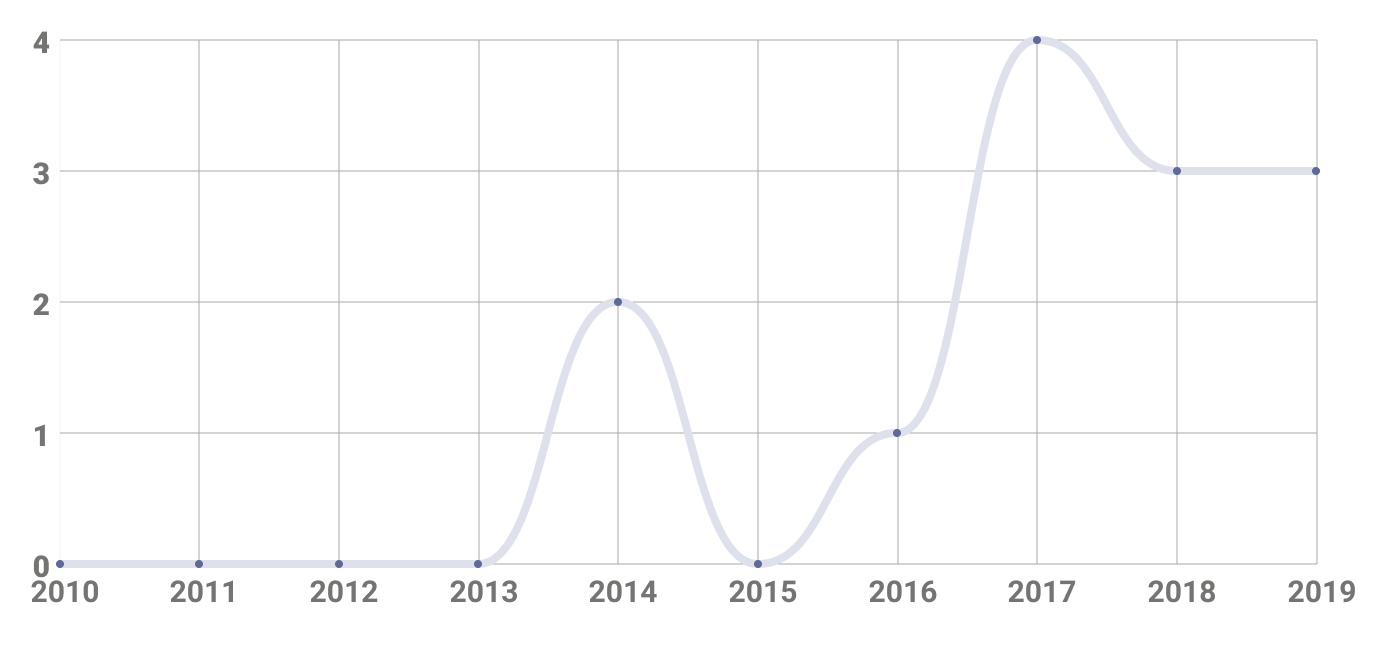
\includegraphics[scale=0.18]
        {Figures/publication_years.png}}
    \caption{\label{fig:publication_years}Identified studies by year}
\end{figure}

\subsubsection{Venue}

The International Requirements Engineering Conference is identified as the main source for the publication of articles of this matter, as four articles were published in proceedings of this congress. Regarding the remaining studies, their publication was conducted in different conferences or journals as seen in Table \ref{tab:studies}.

\subsubsection{Shared References}

All the references made in the studies were collected and compared, thus it was possible to identify the ten most cited studies \cite{Cleland-Huang2006, Cleland-Huang2007, Slankas2013, Glinz2007, Zhang2011AnES, 8049171, 8049172, Knauss2012, Maalej2016, Yang2015}. The most frequent reference was the study by Cleland-Huang et al. in 2006 \cite{Cleland-Huang2006}. Moreover, this article is identified by the studies that refer to it, as one of the earliest applications of machine learning for automated requirements classification. It was also found that more studies among the ten most frequent are authored by Cleland-Huang \cite{Cleland-Huang2007, Knauss2012}. It should be noted that \cite{8049172} and \cite{8049171}, found in the systematic review process, are also among the most cited. Figure \ref{fig:references} shows the frequency with which these studies were cited.

\begin{figure}[!htbp]
    \center{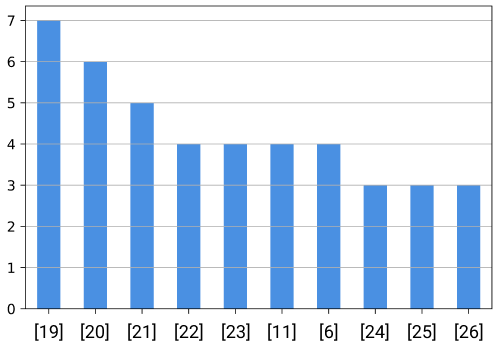
\includegraphics[scale=0.4]
        {Figures/references.png}}
    \caption{\label{fig:references}Top 10 most cited studies}
\end{figure}

\subsubsection{Language Processing and Topic Modeling}

Following the data extraction, the content was analyzed using the Gensim library for text analysis and visualization \cite{rehurek_lrec}. For this process, the full-text was collected via the transcribed version on the studies' download page. In case it was not available, the extraction was done manually. For this analysis, images, tables, equations, as well as their corresponding captions were excluded.

Once gathered the textual content, it was possible to plot a word cloud with the most frequent terms and bigrams throughout all the studies analyzed. In this kind of visualization, the font size represents the frequency with which a bigram or individual term appeared \cite{Cui2010}. In Figure \ref{fig:wordcloud} it is possible to visualize this representation.

\begin{figure}[!htbp]
    \center{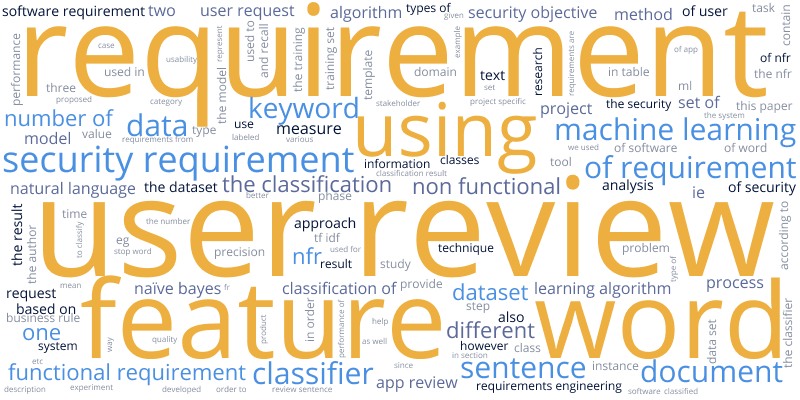
\includegraphics[scale=0.31]
        {Figures/wordcloud.png}}
    \caption{\label{fig:wordcloud}Word cloud of the most frequent terms in the identified studies}
\end{figure}

As a result of this representation, it can be determined that the most frequent terms throughout the studies analyzed were \quotes{requirement}, \quotes{user review}, \quotes{feature} and \quotes{word} and to a lesser extent \quotes{security requirement}, \quotes{machine learning} and \quotes{classifier}.

In addition, a topic modeling process was carried out using the LDA algorithm (Latent Dirichlet Allocation), similar to the process conducted in the systematic review on \cite{Sun2017}. The configuration was set to find four different topics. As a result, the figure \ref{fig:topic_wordcloud} shows another word cloud, in this case, with the most frequent terms of each topic located. It is important to emphasize that it is possible for a term to intersect in more than one topic, especially with very frequent words such as \quotes{requirement}.

\begin{figure}[!htbp]
    \center{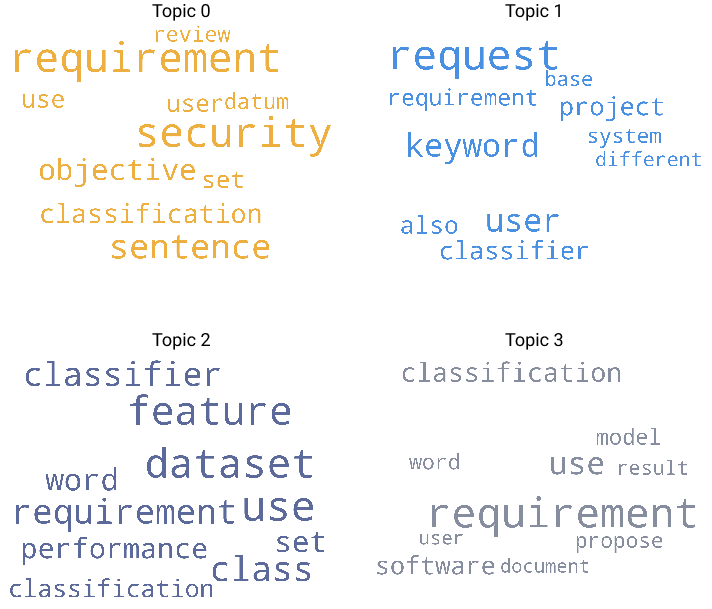
\includegraphics[scale=0.35]
        {Figures/topic_wordcloud.png}}
    \caption{\label{fig:topic_wordcloud}Word cloud of the most frequent terms by topic}
\end{figure}

With the generated LDA model, it is possible to identify the value or weight of a word concerning the topic in which it is found. Thus, Figure \ref{fig:topics_wordcount} presents the relationship between each term and the topic to which it belongs, showing its frequency and weight among each cluster. The textual analysis, the studies' data, and search results can be accessed for replication purposes in the project's repository.\footnote{https://github.com/quality-attributes/systematic-review}

\begin{figure}[!htbp]
    \center{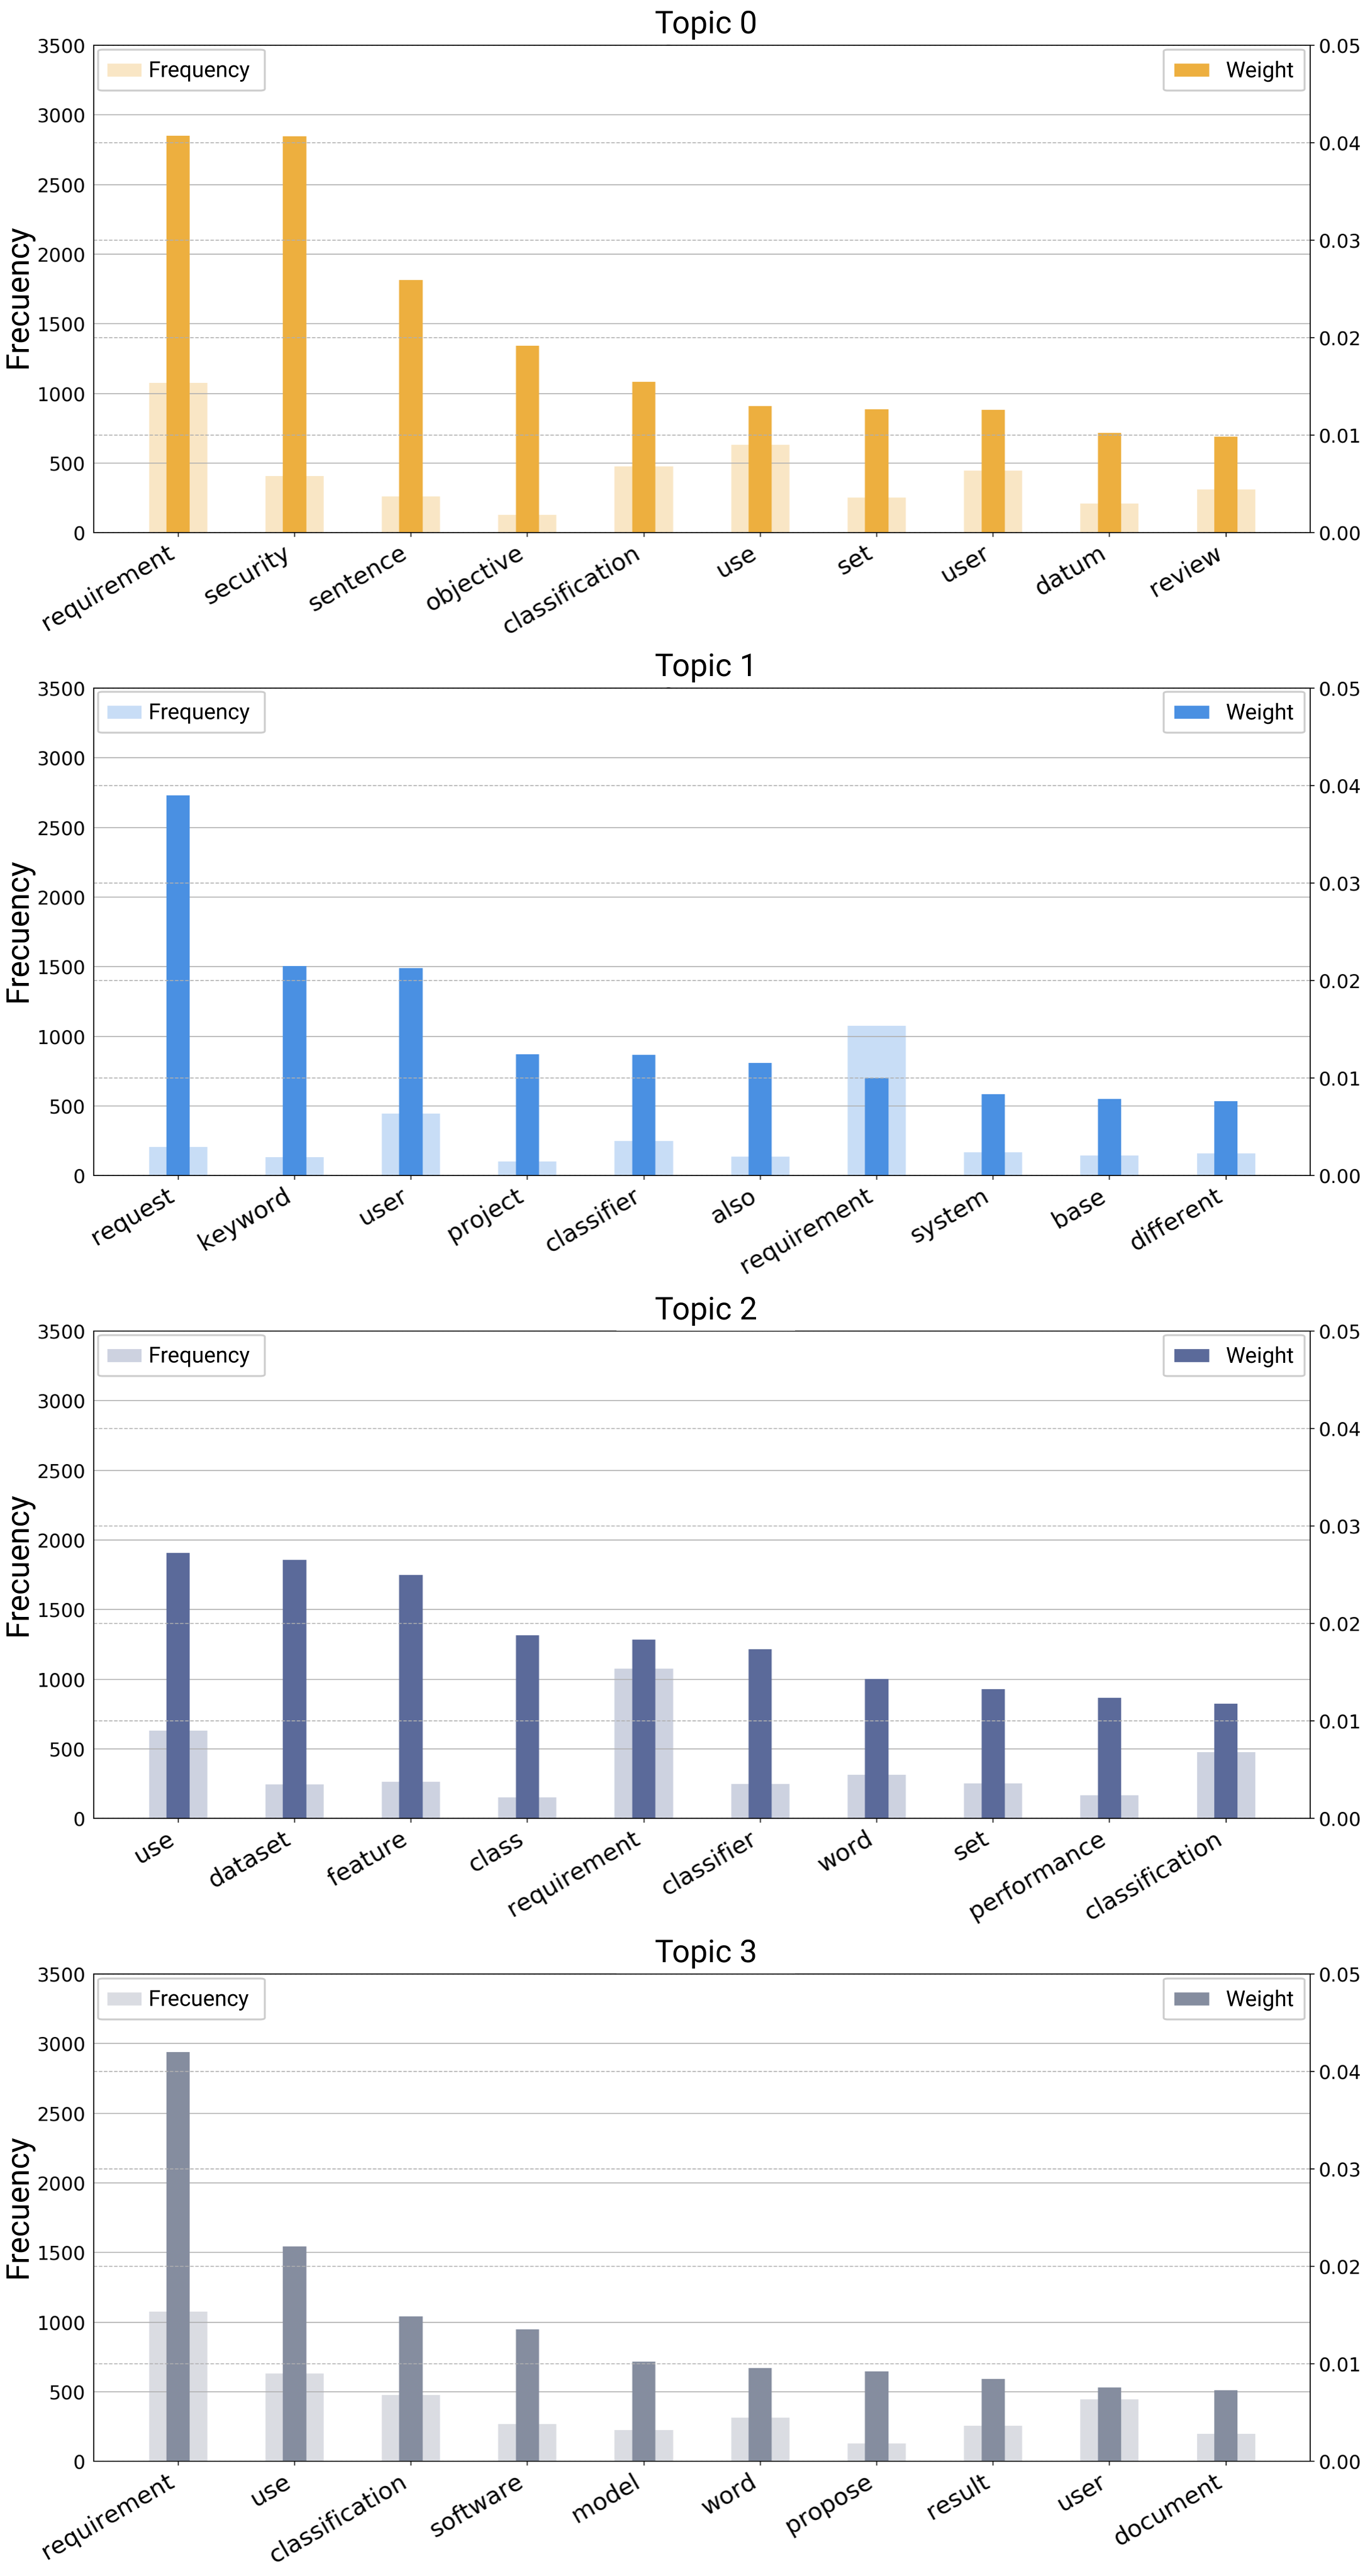
\includegraphics[scale=0.115]
        {Figures/topics_wordcount.png}}
    \caption{\label{fig:topics_wordcount}Frequency and weight of the most common terms in the identified topics}
\end{figure}

\subsection{Data Synthesis}

\subsubsection{RQ1: Which machine learning algorithms have been adopted to classify requirements?}

The study developed by Sharma, Bhatia, and Biswas \cite{6779538} consists of the application of four machine learning algorithms to identify content related to business rules in different academic documents. In this regard, they implemented algorithms such as Minimum Sequential Optimization (SMO), Bayesian Networks, Random Forest, and Naïve Bayes. His approach required different experts to perform the manual classification of documents from different domains for the models' training. Later sections discuss training documents and evaluations.

On the other hand, Abad et al. \cite{8049172} implement the J48 algorithm for decision trees in order to classify requirements sentences into Functional Requirements (FR) and Non-Functional Requirements (NFR). Plus, within the scope of non-functional requirements, they extended their classifications in 11 subcategories: Availability (A), Look \& Feel (LF), Maintainability (MN), Operability (O), Performance (PE), Scalability (SC), Security (SE), Usability (US), Fault Tolerance (FT), and Portability (PO); (b) one constraint category: Legal \& Licensing (L). It is important to note that these implementations required a natural language (NL) preprocessing procedure to fit the requirements' specific notation. The classification of NFR subcategories applied three classification approaches by topic modeling, clustering, and Naïve Bayes. In the classification by topic modeling, they implemented both the Latent Dirichlet Allocation (LDA) and Biterm Topic Model (BTM) algorithms, to establish relationships based on the occurrence of certain words.

Turning to the previous classifications, Baker et al. \cite{8754214} apply machine learning techniques from a different perspective. Using the same database, with the addition of another one featured in a data challenge, a model was created to classify only five categories: maintainability, operability, performance, security, and usability. The approach implements two types of neural networks for this study, Artificial Neural Networks (ANN) with a hidden layer and a Convolutional Neural Networks model trained through the bag-of-words natural language processing method.

Using the same dataset Dekhtyar and Fong \cite{8049170} classified FR and NFR, as well as security-related requirements. However, different NL preprocessing methods were used for this study, such as Term Frequency-Inverse Document Frequency (TF-IDF) and word2vec. The models implemented were a Convolutional Neural Network and Naïve Bayes classifier.

With the same scope for security requirements, the study conducted by Riaz et al. \cite{6912260} focused on identifying this kind of security-related documents. Within its classification, 6 security concerns are identified that are explored in requirements documentation: confidentiality, integrity, identification \& authentication, availability, accountability, and privacy. Consequently, their approach implements NL processing by TF-IDF and classifies through a K-Nearest Neighbor model that is able to identify and suggest templates for the proper drafting of security requirements.

On the other hand, and related to classifiers applied to user reviews, Wang et al. \cite{Wang:2018:ACI:3239235.3267428} trained different machine learning models to test a hypothesis: if the implementation of app changelogs can improve the performance of the classifiers. Thus, their study focuses on classifying user reviews of different applications available in app stores, such as WhatsApp, iBooks, and TripAdvisor. They compared their classifiers' performance by training with and without this additional documentation. Given the nature of the type of comments that are published in reviews, their study only focuses on identifying 6 categories of requirements: Usability, Reliability, Portability, Performance, FR, and Others. Supported by NLP techniques such as stopwords removal, stemming and lemmatization, different classification models are trained: Naïve Bayes, Bagging, J48, and K Nearest Neighbor. Even though their experimental results do not show a considerable improvement in the classification, their study identifies the Naïve Bayes model as the most capable for future studies of this nature.

In general, Table \ref{tab:algorithms} shows the frequency of the ML algorithms identified in the bibliography found. In it, the Naïve Bayes, J48, and K Nearest Neighbor classifiers stand out as the most widely used for the classification of software requirements.


\begin{table}[!htbp]
% table caption is above the table
\caption{Frequency and studies of the identified machine learning algorithms}
\label{tab:algorithms}       % Give a unique label
% For LaTeX tables use
\begin{tabular}{p{3.4cm}p{1cm}p{3cm}}
\hline\noalign{\smallskip}
Model & Frequency & Studies  \\
\noalign{\smallskip}\hline\noalign{\smallskip}
Naive Bayes & 7 & \cite{6779538,8049172,8049170,Wang:2018:ACI:3239235.3267428,LI2018108,Taj:2019:ADM:3328833.3328837,Lu:2017:ACN:3084226.3084241}\\
J48 & 4 & \cite{8049172,Wang:2018:ACI:3239235.3267428,7732349,Lu:2017:ACN:3084226.3084241}\\
K Nearest Neighbor & 3 & \cite{6912260,Wang:2018:ACI:3239235.3267428,LI2018108}\\
Random Fores & 2 & \cite{6779538,8049171}\\
Convolutional Neural Networks & 2 & \cite{8754214,8049170}\\
Bagging & 2 & \cite{Wang:2018:ACI:3239235.3267428,Lu:2017:ACN:3084226.3084241}\\
SMO & 1 & \cite{6779538}\\
Bayesian Network & 1 & \cite{6779538}\\
K-means & 1 & \cite{8049172}\\
LDA & 1 & \cite{8049172}\\
BTM & 1 & \cite{8049172}\\
Artificial Neural Networks & 1 & \cite{8754214}\\
Adaptive Boost & 1 & \cite{8049171}\\
Extra Tree & 1 & \cite{8049171}\\
Gradient Boosting & 1 & \cite{8049171}\\
Support Vector Machine & 1 & \cite{LI2018108}\\
Stochastic Gradient Descent Classifier & 1 & \cite{8590177}\\
Decision Tree & 1 & \cite{Taj:2019:ADM:3328833.3328837}\\

\noalign{\smallskip}\hline
\end{tabular}
\end{table}

\subsubsection{RQ2: What metrics have been used to measure the performance of those algorithms?}

Regarding the means for the machine learning model evaluation, a consensus is identified on three specific metrics: Precision, Recall, and F-Score or F1. 
These metrics are related to model testing, comparing the actual result with the one predicted by the model. The Precision is described as:

\[ Precision = \frac{TP}{TP + FP} \]

Being $TP$ the True Positives, the times the model predicted the right answer, and $FP$ the times that False Positives occurred, meaning a misclassification. However, this metric is calculated concerning a specific class. On the other hand, the Recall metric is expressed as:

\[ Recall = \frac{TP}{TP + FN} \]

Also known as \textit{Sensitivity}, this metric shows the number of right classifications, compared with the misclassification in a different class. Finally, the F-Score describes the relation between Precision and Recall.

\[ F1 = 2\times\frac{Precision\times Recall}{Precision + Recall} \]

Although these metrics are calculated in all the studies identified, excluding the survey conducted in \cite{8719411}, the way they are compared to the original database differs. In some studies, a process of cross-validation is performed, where a series of subsamples or folds is extracted in order to split the dataset into training and test sets, the resulting metrics are the average metrics for each fold \cite{Mitchell:1997:ML:541177}. However, the split between training and test set can be done once and before the training process is performed, in some cases extracting a subsample from the original database, or comparing to a different source in others.

\subsubsection{RQ3: What kind of software projects have been used to train those algorithms?}

During the review, articles were identified that trained their classification models with related databases. Specifically, two databases were adopted by more than one study.

The case of the TERA-PROMISE database \cite{Sayyad-Shirabad+Menzies:2005} consists of 625 functional (FR) and non-functional requirements (NFR) all of them written in requirement notation. Hence, each proposal that adopts it \cite{8719411,7732349,Taj:2019:ADM:3328833.3328837,8049172,8590177} implies text preprocessing.
This database is also divided into sub-categories of non-functional requirements: Availability (A), Look \& Feel (LF), Maintainability (MN), Operability (O), Performance (PE), Scalability (SC), Security ( SE), Usability (US), Fault Tolerance (FT), and Portability (PO); (b) one constraint category: Legal \& Licensing (L). TERA-PROMISE is also referenced within the International Requirements Engineering Conference 2017 Data Challenge, among other databases. Thus different studies focused on their analysis, resulting in papers featured in the conference \cite{8049170,8049171,8049172,8754214}.

Additionally, some studies carried out their training with information from available requirements documentation, such as Software Requirements Specifications (ERS) or domain-specific documents \cite{6779538,6912260}. On the other hand, the analysis of user reviews in search of requirements-related information seemed to be a topic of interest, either from application stores \cite{Taj:2019:ADM:3328833.3328837,LI2018108} or from crowdsourcing sites \cite{Taj:2019:ADM:3328833.3328837,LI2018108}. In the case of these content extraction procedures, prior labeling was required to achieve the training of the classification model. It should be noted that studies were found that performed their training with more than one database.

\begin{figure}[!htbp]
    \center{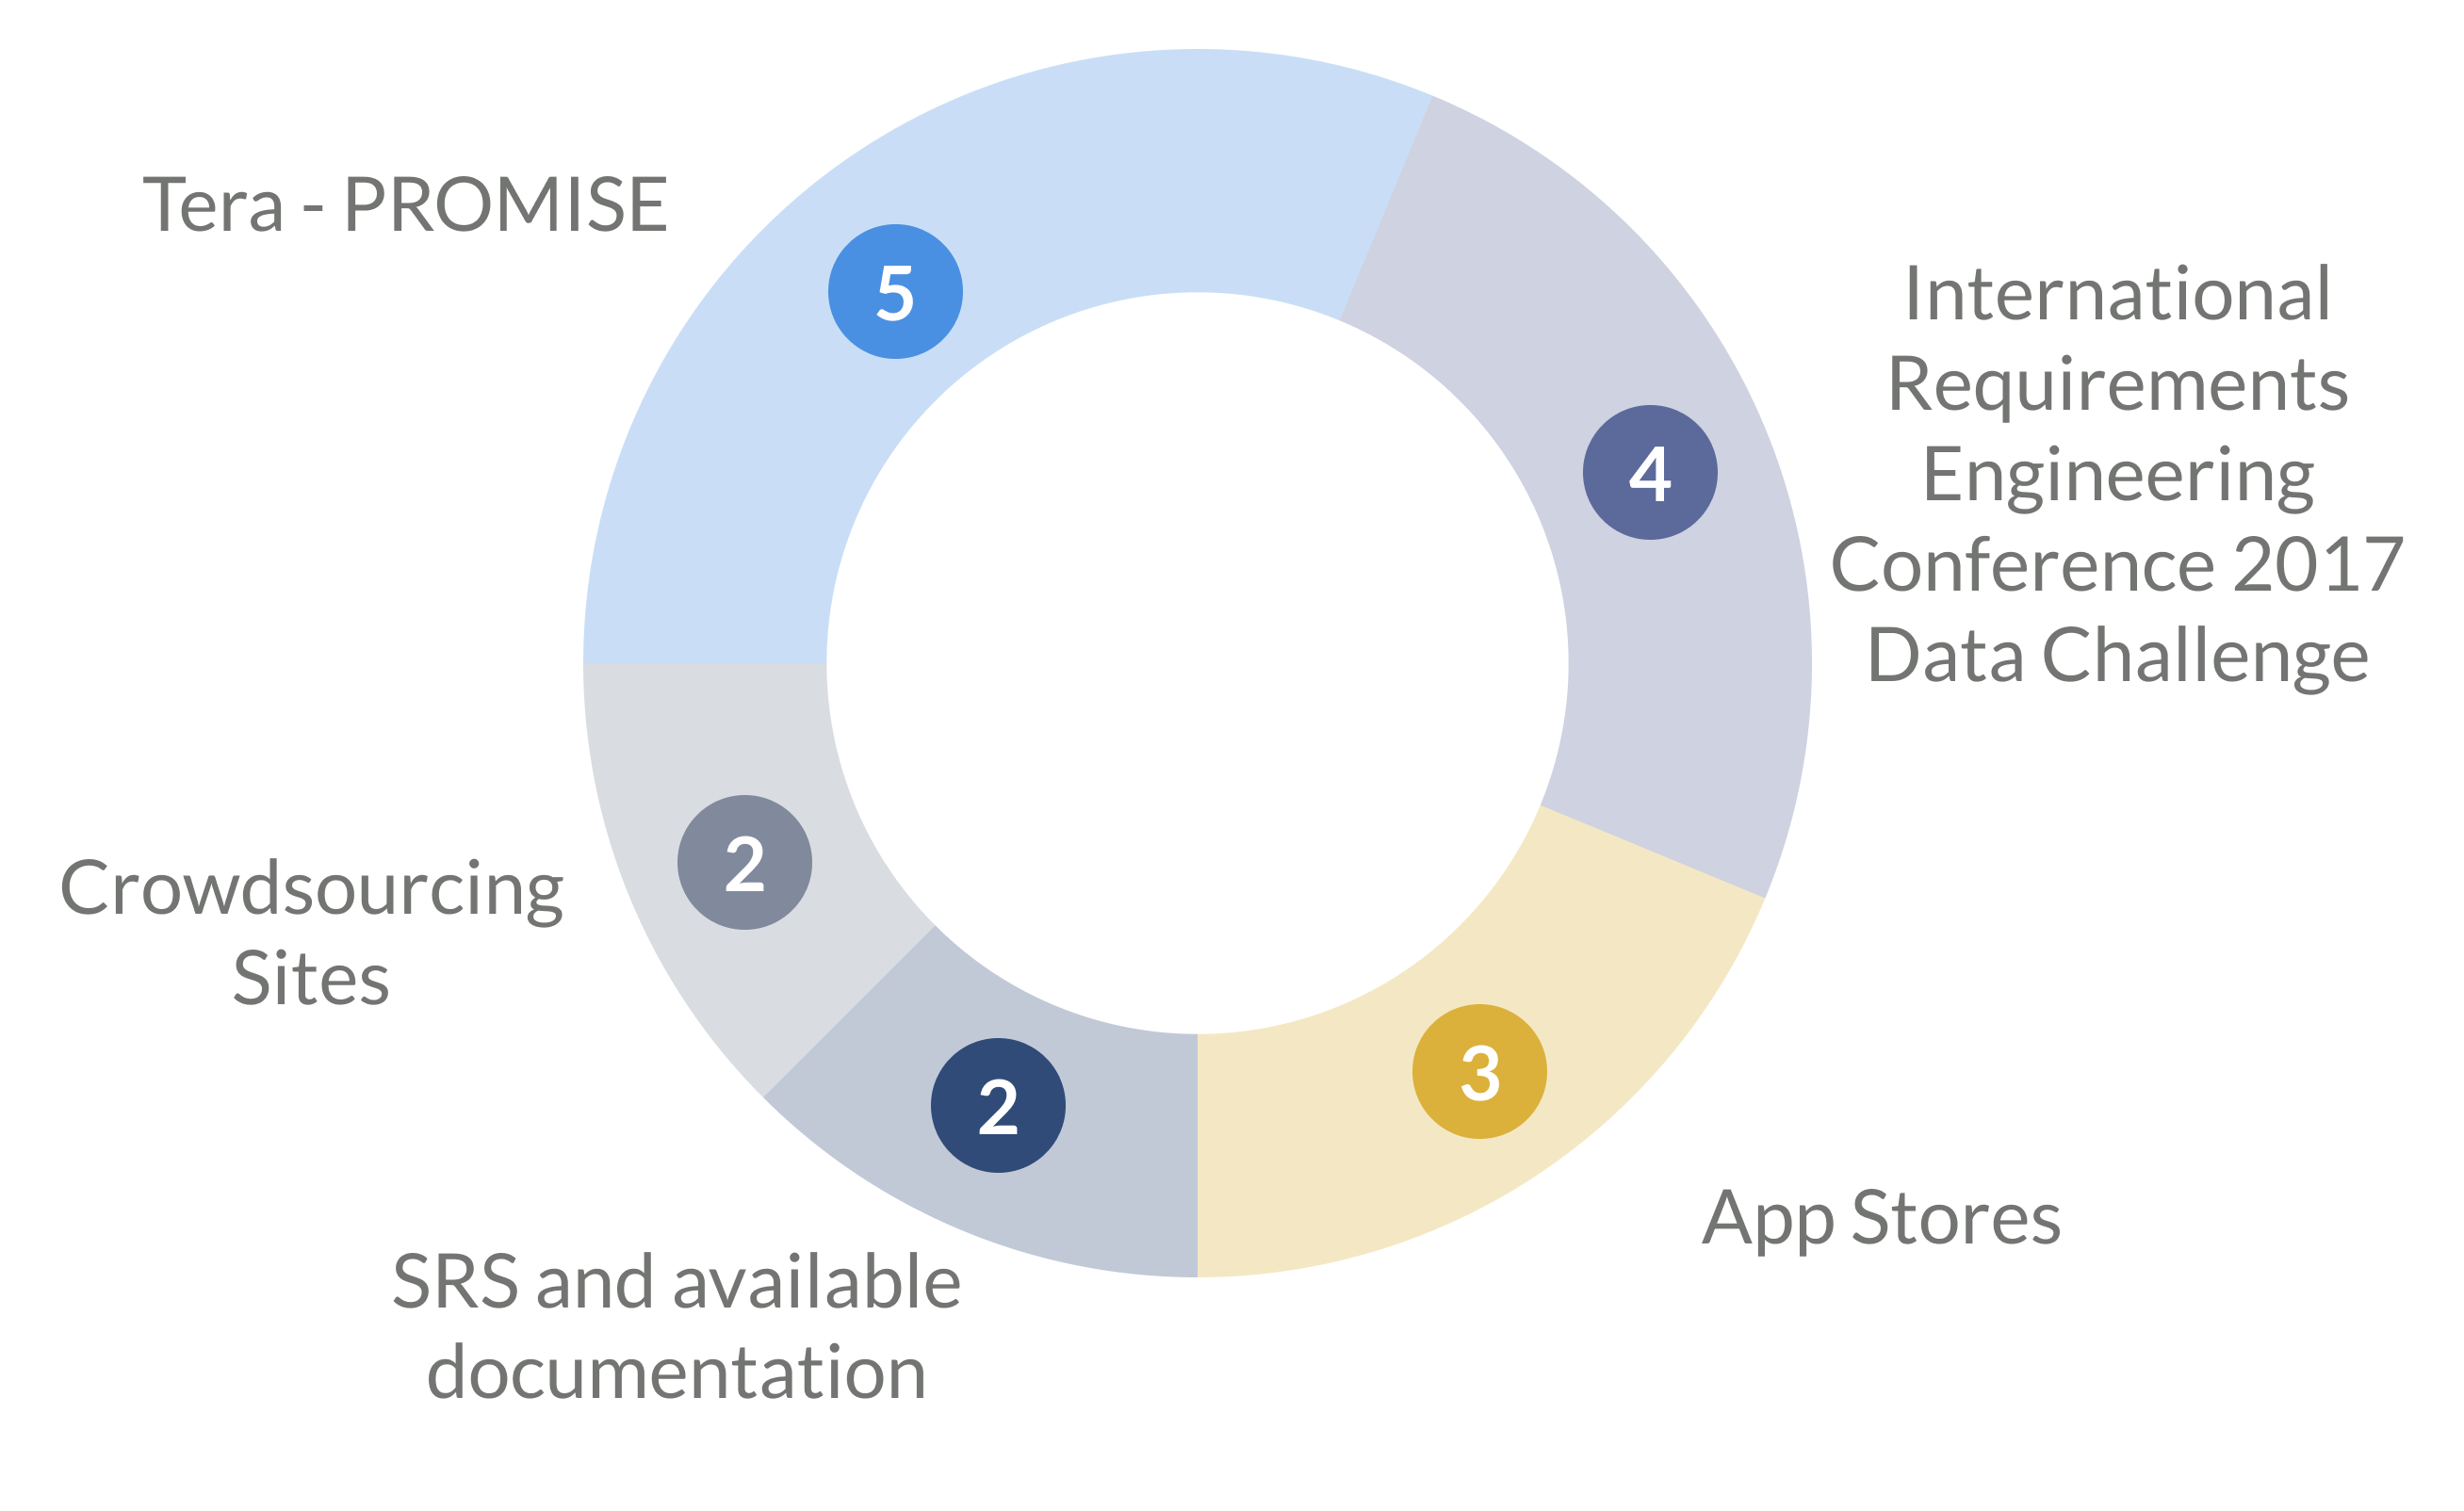
\includegraphics[scale=0.09]
        {Figures/training.png}}
    \caption{\label{fig:training}Data sources used to train the models featured in the identified studies}
\end{figure}

\subsubsection{RQ4: Which requirements categories are the most frequent to train those algorithms?}

Once the target requirements in the studies have been identified, the comparison between them is shown in Figure \ref{fig:categories_freq}. It is worth highlighting that the dichotomy between Functional and Non-Functional Requirements and the subcategories of the latter are the most recurring category-searches in the articles consulted. Something to note is that the search for this category of requirement is frequently focused on requirements associated with Quality Attributes. Although this classification was not carried out by searching all the categories described in the ISO 25010 standard \cite{ISO25010}, articles were found that did so partially, or even only focused on classifying a specific quality attribute such as security \cite{7732349,6912260}.

\begin{figure}[!htbp]
    \center{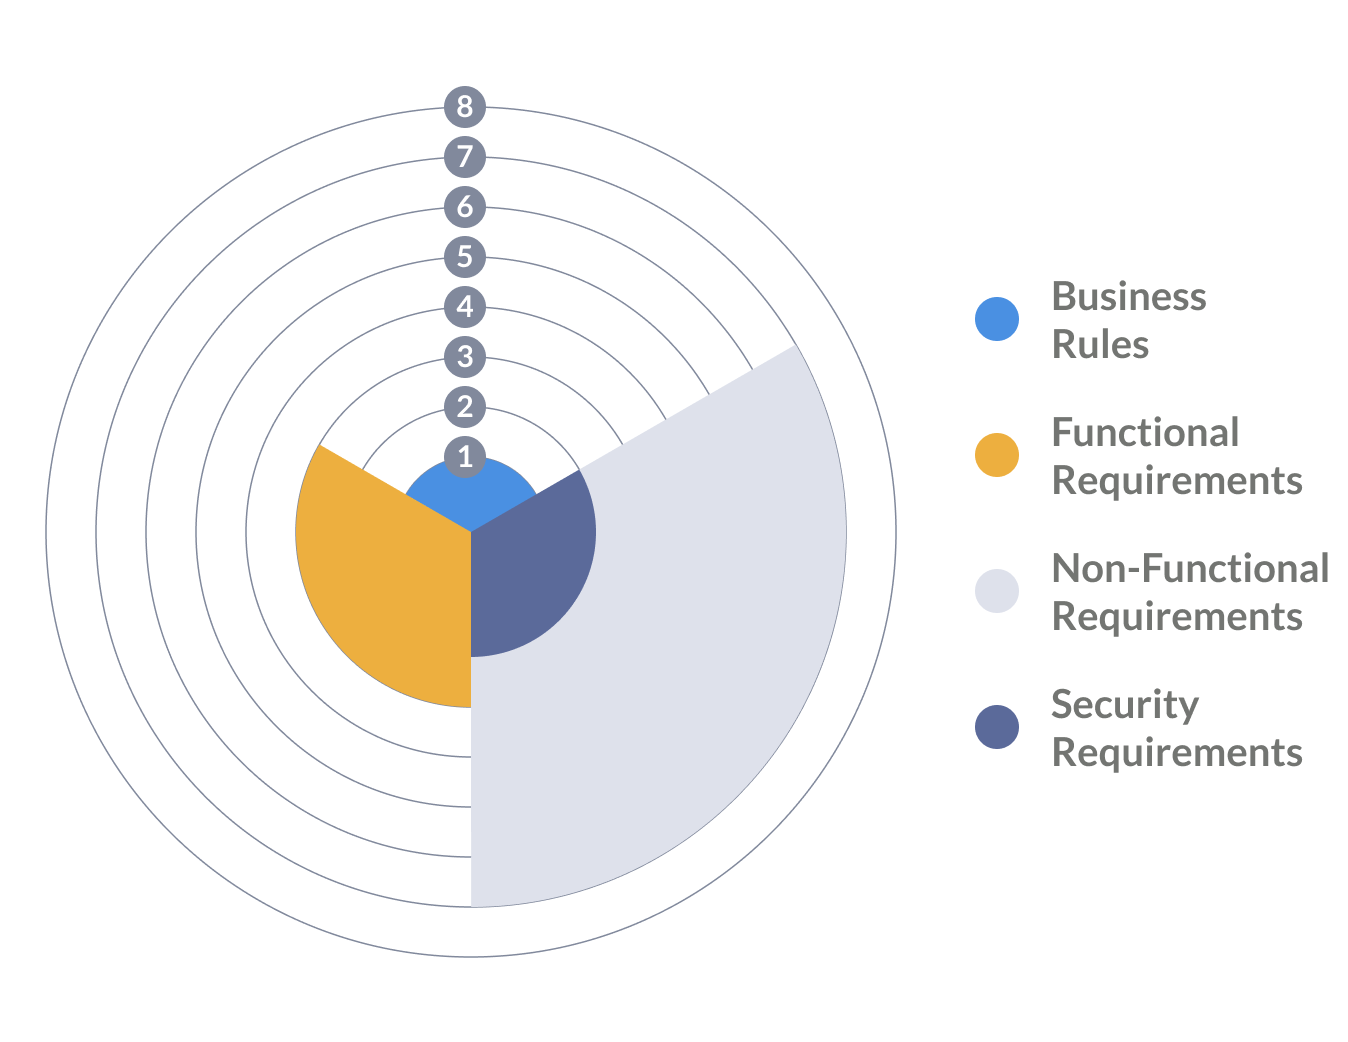
\includegraphics[scale=0.18]
        {Figures/categories_freq.png}}
    \caption{\label{fig:categories_freq}Target requirements categories searched in the studied papers}
    
\end{figure}

In Figure \ref{fig:categories_freq}, the entries counted as Functional Requirements are related to studies that focused only on classifying whether a document was associated to this category or not, without further analysis in the latter case.

\section{Discussion}
\label{discussion}

Automatic software requirements classification represents an area of increasing interest for Requirement Engineering. Recent advances regarding the application of machine learning techniques to classify these requirements were identified in the present study. Based on the results obtained, areas of opportunity and topics of interest are identified concerning this matter. After reading the articles found, \cite{Cleland-Huang2006} is identified as one of the precursor studies on the subject, so it is proposed to extend the years of searching for future literature reviews, to increase the scope of studies. Concerning the spread of these applications, it was found that the most suitable venue for publishing these studies was the International Requirements Engineering Conference, where several studies were published.

Although several studies that address the use of machine learning in the Requirements Engineering area were found, this paper led to the realization that most of the studies regarding automated requirements classification are meant for academic purposes, despite the results found in practical implementations. Regarding the topics of interest, it was found that one of the applications of most comprehensive resonance is the classification of requirements applied to user reviews. 

\section{Conclusions}
\label{conclusions}

Motivated by the novel applications of machine learning in Requirements Engineering, this study aimed to identify the use of these techniques for classifying software requirements. It has been found that there are several proposals for this topic. Regarding the algorithms chosen, several of the studies addressed the use of models such as Naïve Bayes and J48 classifiers. Furthermore, a wide variety of machine learning algorithms were explored in the available literature for requirements classification, implying several preprocessing approaches for processing the text. The assessment of these models is focused on the relation between precision, recall, and F-Score. Nevertheless, the studies found are mostly focused on academic purposes, addressing this topic by using structured requirements databases, rather than natural language. As it was previously stated, an increasing interest in user reviews represents an area available for future research. Finally, it was concluded that most of the studies focus their efforts on classifying functional and non-functional requirements, especially requirements associated with quality attributes.

\bibliographystyle{IEEEtran}
\bibliography{references}

\end{document}
